% Options for packages loaded elsewhere
\PassOptionsToPackage{unicode}{hyperref}
\PassOptionsToPackage{hyphens}{url}
%
\documentclass[
]{book}
\usepackage{lmodern}
\usepackage{amsmath}
\usepackage{ifxetex,ifluatex}
\ifnum 0\ifxetex 1\fi\ifluatex 1\fi=0 % if pdftex
  \usepackage[T1]{fontenc}
  \usepackage[utf8]{inputenc}
  \usepackage{textcomp} % provide euro and other symbols
  \usepackage{amssymb}
\else % if luatex or xetex
  \usepackage{unicode-math}
  \defaultfontfeatures{Scale=MatchLowercase}
  \defaultfontfeatures[\rmfamily]{Ligatures=TeX,Scale=1}
\fi
% Use upquote if available, for straight quotes in verbatim environments
\IfFileExists{upquote.sty}{\usepackage{upquote}}{}
\IfFileExists{microtype.sty}{% use microtype if available
  \usepackage[]{microtype}
  \UseMicrotypeSet[protrusion]{basicmath} % disable protrusion for tt fonts
}{}
\usepackage{xcolor}
\IfFileExists{xurl.sty}{\usepackage{xurl}}{} % add URL line breaks if available
\IfFileExists{bookmark.sty}{\usepackage{bookmark}}{\usepackage{hyperref}}
\hypersetup{
  pdftitle={Dragons Throughout Chinese Arts},
  pdfauthor={Dragon team},
  hidelinks,
  pdfcreator={LaTeX via pandoc}}
\urlstyle{same} % disable monospaced font for URLs
\usepackage{longtable,booktabs}
\usepackage{calc} % for calculating minipage widths
% Correct order of tables after \paragraph or \subparagraph
\usepackage{etoolbox}
\makeatletter
\patchcmd\longtable{\par}{\if@noskipsec\mbox{}\fi\par}{}{}
\makeatother
% Allow footnotes in longtable head/foot
\IfFileExists{footnotehyper.sty}{\usepackage{footnotehyper}}{\usepackage{footnote}}
\makesavenoteenv{longtable}
\usepackage{graphicx}
\makeatletter
\def\maxwidth{\ifdim\Gin@nat@width>\linewidth\linewidth\else\Gin@nat@width\fi}
\def\maxheight{\ifdim\Gin@nat@height>\textheight\textheight\else\Gin@nat@height\fi}
\makeatother
% Scale images if necessary, so that they will not overflow the page
% margins by default, and it is still possible to overwrite the defaults
% using explicit options in \includegraphics[width, height, ...]{}
\setkeys{Gin}{width=\maxwidth,height=\maxheight,keepaspectratio}
% Set default figure placement to htbp
\makeatletter
\def\fps@figure{htbp}
\makeatother
\setlength{\emergencystretch}{3em} % prevent overfull lines
\providecommand{\tightlist}{%
  \setlength{\itemsep}{0pt}\setlength{\parskip}{0pt}}
\setcounter{secnumdepth}{5}
\usepackage{booktabs}
\ifluatex
  \usepackage{selnolig}  % disable illegal ligatures
\fi
\usepackage[]{natbib}
\bibliographystyle{apalike}

\title{Dragons Throughout Chinese Arts}
\author{Dragon team}
\date{\texttt{December\ 18,\ 2020}}

\begin{document}
\maketitle

{
\setcounter{tocdepth}{1}
\tableofcontents
}
\hypertarget{motivation}{%
\chapter*{Motivation}\label{motivation}}
\addcontentsline{toc}{chapter}{Motivation}

The \textbf{bookdown} package can be installed from CRAN or Github:

Remember each Rmd file contains one and only one chapter, and a chapter is defined by the first-level heading \texttt{\#}.

To compile this example to PDF, you need XeLaTeX. You are recommended to install TinyTeX (which includes XeLaTeX): \url{https://yihui.org/tinytex/}.

\hypertarget{intro}{%
\chapter*{Introduction}\label{intro}}
\addcontentsline{toc}{chapter}{Introduction}

\hypertarget{ancient}{%
\chapter*{Dragon Art in Ancient China}\label{ancient}}
\addcontentsline{toc}{chapter}{Dragon Art in Ancient China}

Discovered at Sanguan Dianzi in Liaoning province, from the Neolithic Hongshan Culture,this jade ``Pig-Dragon'' ornament is one of the first representations of the Dragon figure that we see in Chinese art culture. Neolithic cultures usually derived their art inspiration from nature itself, they still did not have a concrete sense of religion, nor the concept of longevity attached to the dragon. This type of artifact was found buried in stone ritual structures, giving them a ritualistic meaning (Ebrey).
Called a ``Pig- Dragon'' because of the similar form of the snout to that of a pig. This Dragon also has a long body characterized by a Chinese Dragon, yet it is in a ring shape. To give this piece of jade this ring dragon shape neolithic villagers most had used sand and days to polish.

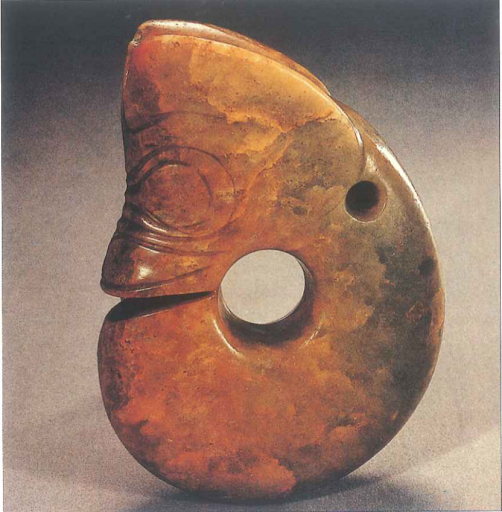
\includegraphics[width=1\textwidth,height=\textheight]{images/1. Jade_Pig_Dragon.png}

\href{}{(c.~3500 BC., Hongshan Culture, Neolithic period). Pig-Dragon Ring; Jade. The National Museum of China, Beijing, China.}

\hypertarget{artifact3}{%
\chapter*{Artifact 3}\label{artifact3}}
\addcontentsline{toc}{chapter}{Artifact 3}

We describe our methods in this chapter.

\hypertarget{artifact4}{%
\chapter*{Artifact 4}\label{artifact4}}
\addcontentsline{toc}{chapter}{Artifact 4}

Some \emph{significant} applications are demonstrated in this chapter.

\hypertarget{example-one}{%
\section{Example one}\label{example-one}}

\hypertarget{example-two}{%
\section{Example two}\label{example-two}}

\hypertarget{Dragon_Paintings}{%
\chapter*{Dragon Paintings in the Song and Yuan Dynasties}\label{Dragon_Paintings}}
\addcontentsline{toc}{chapter}{Dragon Paintings in the Song and Yuan Dynasties}

Placeholder

\hypertarget{the-emergence-of-dragon-paintings-in-the-song-dynasty}{%
\section*{The emergence of Dragon paintings in the Song Dynasty}\label{the-emergence-of-dragon-paintings-in-the-song-dynasty}}
\addcontentsline{toc}{section}{The emergence of Dragon paintings in the Song Dynasty}

\hypertarget{dragon-paintings-as-bearers-of-rain}{%
\section*{Dragon Paintings as Bearers of Rain}\label{dragon-paintings-as-bearers-of-rain}}
\addcontentsline{toc}{section}{Dragon Paintings as Bearers of Rain}

A
\# References \{-\}

\hypertarget{artifact7}{%
\chapter*{Artifact 7}\label{artifact7}}
\addcontentsline{toc}{chapter}{Artifact 7}

Some \emph{significant} applications are demonstrated in this chapter.

\hypertarget{example-one}{%
\section{Example one}\label{example-one}}

\hypertarget{example-two}{%
\section{Example two}\label{example-two}}

  \bibliography{book.bib,packages.bib}

\end{document}
